Questo capitolo ha lo scopo di illustare la soluzione proposta, i passaggi intermedi ed i regionamenti logici che mi hanno portato ad elaborare la soluzione finale.

Sarà anzitutto chiarito il perchè del linguaggio \textit{Rust}, definendo le sue particolarità ed i sui punti critici, poi saranno illustrate le pubblicazioni utilizzate per migliorare le soluzioni iniziali, infine verrà eseguita un'analisi dei tempi di calcolo della soluzione definitiva.

\section{Perchè il Linguaggio Rust}
Il linguaggio Rust è un linguaggio di programmazione sviluppato da Mozilla insieme alla comunità open source per la programmazione di sistemi.

\begin{figure}
    \centering
    
\includegraphics[scale=0.5]{images/rustlang.jpg}
    \caption{Logo del Linguaggio Rust affiancato a quello di Mozilla}
    \label{fig:rustlang1}
\end{figure}

Rust persegue obiettivi di efficienza e sicurezza ed è idoneo allo sviluppo di software concorrente. Sintatticamente simile a \textit{C++}, si differenzia da quest'ultimo a causa del suo meccanismo di salvaguardia della memoria chiamato \textit{Borrow Checker}, che si avvale del design patter \textsc{RAII} (Resource Acquisition Is Initialization) per deallocare le risorse nel caso il loro \textit{Owner} esca di scope \cite{10.5555/3271463}.

Rust non permette l'utilizzo di \textit{null pointer} e \textit{Dangling Reference} che devono essere, in alcuni casi, esplicitamente validati tramite \textit{lifetime}, ciò lo rende un linguaggio sicuro, infatti è stato utilizzato per scrivere alcuni moduli del browser mozilla e parte di alcuni sistemi operativi, tra cui Android.

Rust è usato in bioinformatica, ma in generale in ambito scientifico, perchè oltre alle caratteristiche sopra elencate, è un linguaggio con una buona espressività, simile a quella di un linguaggio a più alto livello, ma più veloce. Ciò lo rende adeguato allo sviluppo di applicativi che necessitano di una buona velocità d'esecuzione e per utenti che non vogliono perdere tempo con gli errori tipici, ad esempio, del C++. Una pecca di rust è che, in generale, è difficoltoso da imparare \cite{whyrust}. 

\section{Primo Approccio}
Prima di poter lavorare sul problema effettivo, c'è stato un preambolo di circa tre settimane in cui è avvenuta una grossa fase di apprendimento. Dapprima ho imparato il linguaggio Rust, poi ho appreso i costrutti resi disponibili dalle varie librerie per adempiere ai miei compiti. In questa fase ho anche creato il parser di file in formato MAF, che è stato un buon esercizio per apprendere ancora meglio Rust.

Terminato questo preambolo, l'approccio che ho deciso di utilizzare per la costruzione dello splicing graph, è stato quello di scansionare l'allineamento colonna per colonna e costruire il grafo di conseguenza. 

In pratica, si assiste ad una fase di inizializzazione, in cui viene creato il nodo 1 con etichetta \textit{first\_node} e aggiunto al \textit{Path} di ogni trascritto nell'allineamento. 

Il costrutto Path è utile in quanto permette di memorizzare i cammini associati ai vari trascritti in termini di sequenza di nodi, quindi di poter associare ad ogni trascritto un percorso attraverso i vertici che corrisponde alla sua sequenza genomica.

In seguito, per ogni colonna dell'allineamento, si costruisce l'insieme dei simboli contenuti, scartando eventuali indel. Per ogni simbolo si costruisce un nodo la cui etichetta è costituita da simbolo stesso e lo si "Aggancia" correttamente al nodo precedente. Dopo aver portato a termine questa operazione, si aggiunge ogni nodo al o ai Path corretti (vedi figura \ref{fig:SplicingGraphConstructionPhases}).

\begin{figure}
    \centering
    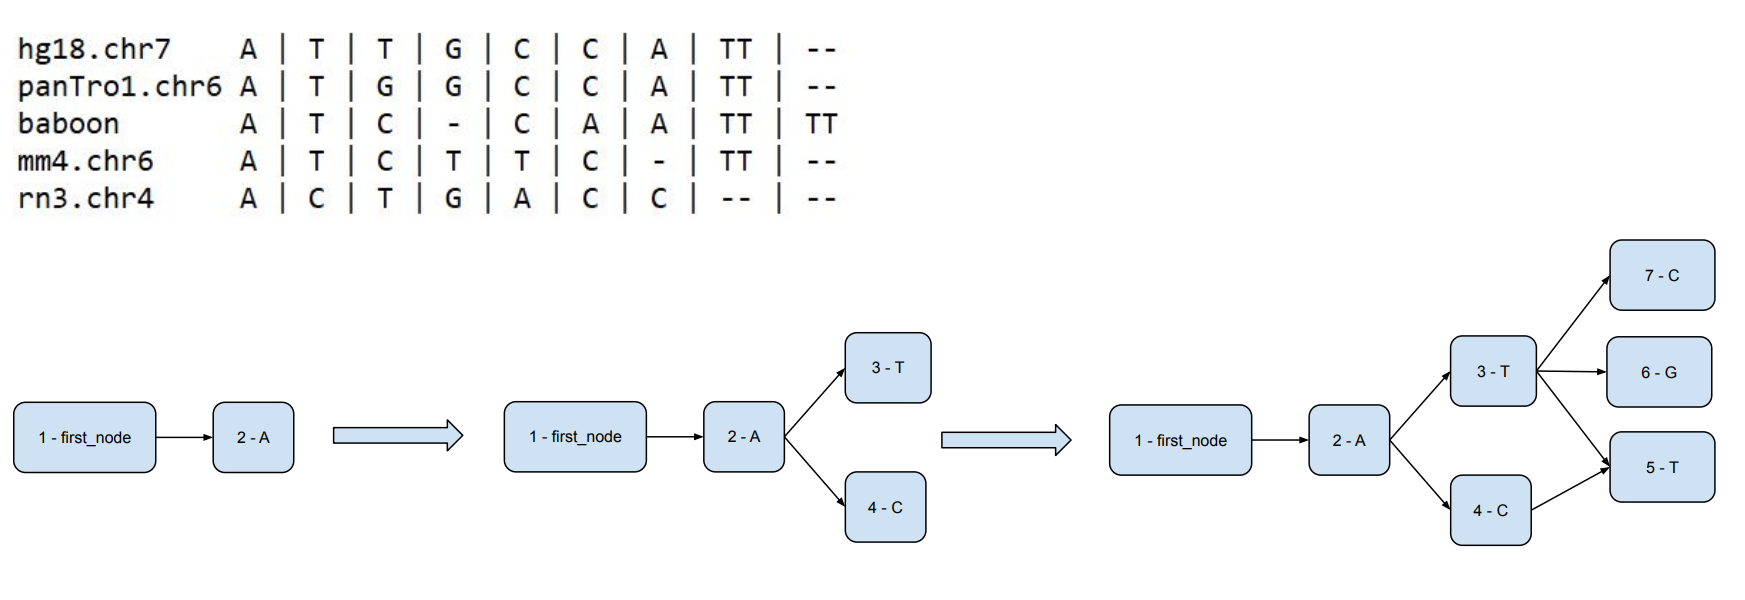
\includegraphics[scale=0.43]{images/Fasi primo approccio.PNG}
    \caption{Le prime tre fasi della costruzione dello Splicing Graph. Vengono prese in considerazione le prime colonne dell'allineamento}
    \label{fig:SplicingGraphConstructionPhases}
\end{figure}

Infine si assiste ad una fase di epilogo in cui tutti i nodi formati nell'ultima iterazione della fase precedente vengono agganciati ad un ultimo nodo etichettato \textit{last\_node} che corrisponde al nodo di fine e unico nodo foglia del grafo.

Come si può inture, questo metodo di creazione dello splicing graph, porta alla creazione di un grafo con un'eccessivo numero di nodi ed un eccessivo numero di percorsi $first\_node \to last\_node$. Ricordo che, dove possibile, è necessario limitare il numero di questi percorsi.

Una soluzione potrebbe essere quella di seguire lo stesso approccio per la costruzione del grafo, ma invece di considerare l'allineamento colonna per colonna, procedere con un partizionamento opportuno per fare sì di creare dei nodi con etichetta di lunghezza maggiore di 1, facendo sì di diminuire i nodi già presenti.

La prossima sezione spiegherà le metodologie utilizzate per l'ottenimento di un partizionamento opportuno.

\section{Metodologie di partizionamento}
Un buon partizionamento, dovrebbe fare in modo di accorpare il più possibile le colonne dell'allineamento, così da diminuire le quantità di nodi e di percorsi $first\_node \to last\_node$. Per assolvere a questo compito, sono utilizzati due approcci, uno di \textit{programmazione Dimanica} e uno \textit{Greedy}, che originariamente sono stati pensati per risolvere il \textit{Founder Sequence Reconstruction Problem}. Entrambi gli approcci sono descritti in \cite{ukkonen}.

\subsection{Concetti Teorici Preliminari}
Ancora una volta saranno presentati alcuni concetti teorici necessari alla comprensione degli metodi utilizzati per la risoluzione del problema.

Sia $\mathbb{C}=\{C_1,C_2,...,C_m\} \subseteq \Sigma^n$ un insieme di sequenze di lunghezza $n$ su un alfabeto $\Sigma$ detti \textit{Ricombinanti}, ogni ricombinante è scritto come $C_i=c_{i1},c_{i1},...,c_{in}$. Un insieme $\mathbb{F}=\{F_1,F_2,...,F_k\} \subseteq (\Sigma \cup \{\textit{-}\})^n$ è chiamato \textit{Insieme dei Fondatori} per
l'insieme $\mathbb{C}$ e ogni $F_i$ è detta sequenza fondatrice se $\mathbb{C}$ ha un \textit{Parsing} in termini di $\mathbb{F}$. 

Ciò significa che ogni $C_i \in \mathbb{C}$ può essere decomposto in una serie di \textit{Frammenti} non vuoti $f_{ih}$ tale che $C_i=f_{i1}f_{i2}...f_{ip_i}$ e ogni $f_{ih}$ occorre un qualche $F \in \mathbb{F}$ nella stessa posizione in cui è presente anche in $C_i$. 

In altre parole, si può riscrivere $F=\alpha f_{ih} \beta$ dove la lunghezza di $\alpha$ è uguale a quella di $|\alpha|=|f_{i1}...f_{ih-1}|$, mentre la lunghezza di $\beta$ è uguale a quella di $|\beta|=|f_{ih+1}...f_{ip_i}|$.

Si assume che il parsing sia \textit{ridotto} nel senso che due successivi frammenti di $f_{ih}$ e $f_{ih+1}$ siano sempre estratti da elementi diversi di $\mathbb{F}$.

In un parsing (ridotto) di $\mathbb{C}$, si dice che un un ricombinante $C_i$ ha un \textit{Punto di crossover} in $j$ se il parse di $C_i$ è  $C_i=f_i...f_hf_{h+1}...f_{p_i}$ e $|f_1...f_h|=j-1$.

\begin{example}
L'insieme dei ricombinanti:
\begin{center}
  \begin{tabular}{ c c c c c c c c c c c c}
    0 & 0 & 1 & 0 & 0 & 0 & 0 & 1 & 0 & 0 & 1 & 1 \\ 
    1 & 1 & 1 & 1 & 1 & 1 & 1 & 0 & 0 & 1 & 1 & 0 \\
    0 & 0 & 1 & 0 & 1 & 1 & 1 & 1 & 0 & 1 & 1 & 0 \\ 
    1 & 1 & 1 & 1 & 0 & 0 & 1 & 0 & 0 & 0 & 1 & 1 \\
  \end{tabular}
\end{center}

L'insieme dei fodatori:
\begin{center}
  \begin{tabular}{ c c c c c c c c c c c c}
    0 & 0 & 1 & 0 & 1 & 1 & 1 & 0 & 0 & 0 & 1 & 1 \\ 
    1 & 1 & 1 & 1 & 0 & 0 & 0 & 1 & 0 & 1 & 1 & 0 \\
  \end{tabular}
\end{center}
\end{example}

\newpage

A questo punto, il nostro problema è quello di trovare il set di fondatori $\mathbb{F}$ di cardinalità minima, nel contempo massimizzare la lunghezza del frammento più corto $\lambda_{min}$ e la lunghezza media dei frammenti $\lambda_{ave}$. Come è intuitivo pensare, questi sono due obiettivi contradditori.

Ciò ci porta alla formalizzazione di due problemi:

\begin{itemize}
    \item Il primo è il \textsc{minimum founder set problem} che consiste nel trovare il set di fondatori $\mathbb{F}$ di cardinalità minima tale che il parse di $\mathbb{}$ in termini di $\mathbb{F}$ abbia $\lambda_{min} > L$ oppure $\lambda_{ave} > L$ per un L dato chiamato \textit{Threshold}.
    
    \item Il secondo è il \textsc{maximum fragment length problem} che consiste nel massimizzare $\lambda_{min}$ e/o $\lambda_{ave}$ sotto la condizione che la cardialità di $\mathbb{F} \leq M $ per un M dato.
\end{itemize}

Al fine di costruire uno Splicing Graph, è sembrato più congeniale, modellare il problema a partire dal \textsc{minimum founder set problem}, in quato si è voluta tenere più bassa possibile la cardinalità di $\mathbb{F}$. Ciò ha porta ad un buon grafo, a cui possono essere fatte ulteriori migliorie.

\subsection{Soluzione di Programmazione Dinamica}
Un algoritmo risolutivo del minimum founder set problem è basato sull'idea di segmentare l'insieme de ricombinanti $\mathbb{C}$ in segmenti disgiunti, in modo da partizionare interamente $\mathbb{C}$. Un segmento $C[j,k]$ è definito come l'insieme si tutte le sottosequenze $c_{ij}...c_{ik}$ dell'insieme dei Ricombinanti. 

Il nostro obiettivo diventa quindi quello di dare un parsing di $\mathbb{C}$ con $\lambda_{min} > L$ per un L dato, tale che la ardinalità massima dei segmenti sia minimizzata, ciò minimimizza anche la cardinalità dell'insieme $\mathbb{F}$ dato che $|\mathbb{F}|=|\max\{C[j,k]\}|$

Si vuole quindi computare:

\begin{equation*}
    M(n)=\min_{s \in S_L}\{|C[j,k]| : |C[j,k]| \in s \} 
\end{equation*}

Dove s è linsieme dei partizionamenti possibili su $\mathbb{C}$.

Quindi $M(n)$ può essere ottenuto valutando $M(L),M(L+1)...M(n),$ nel seguente modo:

Caso base:

\begin{equation*}
    M(L)= |C[1,L]| 
\end{equation*}

Passo Ricorsivo:

\begin{equation*}
    M(j)= \min_{h \leq j-L} \max_{j=L+1,...,n} \{M(h),|C[h+1,j]|\}
\end{equation*}

Il tempo di calcolo per questo approccio è $\mathcal{O}(n^2m)$ dove $n$ è la lunghezza dell'allineamento e $m$ è il numero delle sequenze allineate.

Con l'usuale traceback dell'array di programmazione dinamica,, è possibile giungere al partizionamento corretto.

Questa soluzione non tiene però conto degli indel presenti nelle sequenze. 

E' opportuno o meno contare sottosequenze che presentano solo indel nella cardinalità dei segmenti? o ancora; è opportuno contare le sottosequenze formate solo parzialmente da indel?

Come conseguenza della soluzione greedy presentata nella prossima sezione, sono arrivato alla conclusione che non ha senso il conteggio di una sottosequeza di soli indel nella cardinalità di un segmento. Invece ha senso il conteggio di una sottosequenza formata solo parzialmente da indel.

In generale questa soluzione di programmazione dinamica non restituisce risultati ottimali.

In particolare con allineamenti di sequenze troppo diverse tra di loro, si assiste ad un partizionamento praticamente inesistente, nel senso che, in un caso linite, si verrà a formare un grafo con $n+2$ vertici, con etichette corrispondenti alle intere sequenze in input, che corrispondono alle $n$ sequenze in aggiunta al nodo etichettato $first\_node$ e a quello etichettato $last\_node$.

La soluzione greedy cerca di ovviare a questo problema.

\subsection{Soluzione Greedy}

La soluzione greedy, anch'essa descritta in \cite{ukkonen}, ha come obiettivo quello di trovare il partizionamento con il minor numero di segmenti tale che ogni segmento abbia cardinalità massima $M$.

Tale obiettivo è raggiunto considerando inizialmente $|C[1,k]| \leq M$ poi progressivamente $|C[k+1,k']| \leq M$ fino al termine dell'allineamento, tale che i partizionamenti siano più lunghi possibile.

Questa soluzione è però fin troppo semplicistica, infatti non contempla il fatto che un segmento di cardinalità 1 potrebbe già superare la soglia $M$. 

Che fare in questo caso?

Si potrebbe pensare di scegliere $M$ opporunamente, in modo da non permettere a questo caso di presentarsi. Dovrebbe essere sufficiente inserire un valore di $M \geq \min \{|\Sigma|,n\}$ dove $n$ è il numero delle sequenze e $|\Sigma|$ è la cardinalità dell'alfabeto su cui sono costruite le stringhe.

Questo tipo di soluzione porterebbe però, in alcuni casi, a segmenti troppo lunghi, quindi a non accorpare al meglio l'allineamento.

Al fine di poter mantenere un valore di $M>0$, inizialmente ho pensato di interrompere il segmento nel caso $|C[k,k+1]| > M$. Però ciò portava ad un grafo come quello mostrato in figura \ref{fig:primo_esempio_splicing_graph_greedy}.

\begin{figure}
    \centering
    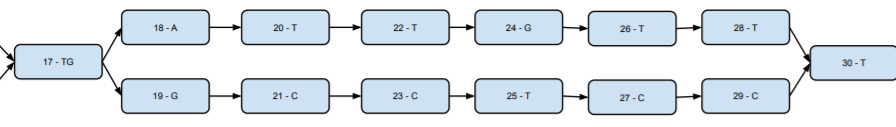
\includegraphics[scale=0.7]{images/greedy1.PNG}
    \caption{Primo Esempio di soluzione greedy. Per comodità, è riportato solo un frammento del grafo}
    \label{fig:primo_esempio_splicing_graph_greedy}
\end{figure}

Logicamente si vorrebbero accorpare i nodi 18, 20, 22, 24, 26, 28 in un unico nodo, così come i vertici 19, 21, 23, 25, 27, 29.

Ciò è possibile se si permette all'algoritmo di partizionamento, in certi casi, di non attenesi al vincolo di cardinalità dei segmenti. I casi in questione sono proprio quelli menzionati in precedenza, infatti se il segmento di cardinalità minima già eccede $M$, allora gli è permesso accorpare più colonne dell'allineamento fino a quando non aumenta ulteriormente di cardinalità, o quando non è possibile formare un nuovo frammento di cardinalità minore. Allora si inizia un nuovo fragmento.

Nel conteggio di cardinalità dei segmenti sono omesse le sottosequenze di sonli indel, esattamente come nell'algoritmo di programmazione dinamica menzionato nella sezione precedente.

Questo "Nuovo" algoritmo greedy permette di formare un grafo come quello in figura \ref{fig:greedy_definitivo}.

\begin{figure}
    \centering
    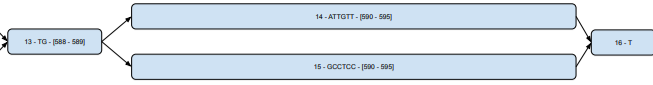
\includegraphics[scale=0.9]{images/greedy2.PNG}
    \caption{Esempio definitivo di soluzione greedy, Per comodità, è riportato solo un frammento del grafo e sono riportati gli indici dell'allineamento corrispondenti alle etichette dei nodi}
    \label{fig:greedy_definitivo}
\end{figure}

\section{Approccio Definitivo}
Tra il primo approccio e l'approccio definitivo si sono susseguiti numerosi tentativi. Per chiarezza espositiva, verranno esposti solo il primo e il definitivo, in modo da non essere troppo prolissi nell'esposizione.

Avendo un partizionamento adeguato, la fase di corstruzione del grafo risulta molto simile a quella del primo approccio. 

La fase di inizializzazione è identica a quella precedentemente descritta, come la fase di terminazione, mentre quella di costruzione vera e propria deve tenere conto che non si ragiona più in termini di siboli, ma in termini di sottostringhe dell'allineamento. A parte questo, il grafo è costruito incrementalmente come mostrato nella figura \ref{fig:SplicingGraphConstructionPhases}.

Il partizionamento è ottenuto tramite la segmentazione greedy. in ogni caso l'utente può utilizzare l'algoritmo di programmazione dinamica.

Il valore si soglia $M$ è impostabile dall'utente, ma è consigliato tenerlo basso per fare in modo di costruire un grafo migliore. Ad esempio, nella figura \ref{fig:greedy_definitivo}, è stato scelto il valore $M=1$.

\section{Tempi di Calcolo}
Fare un'analisi formale dei tempi di calcolo risulterebbe difficile. La fase di preprocessamento delle sequenze, in cui viene estratto il partizionamento, come detto il precedenza, ha tempo $\mathcal{O}(nm)$. 

La vera e propria fase di costruzione prende un tempo che è proporzionale al numero dei segmenti nella partizione creata, alla cardinalità dei segmenti e al numero delle sequenze allineate.




